\par
Avant d’investir des millions de dollars et des centaines d’heures pour 
construire un bâtiment, les propriétaires fonciers doivent savoir si le 
plancher peut supporter le bâtiment en question. Un sous-sol mou et 
rempli d'air peut conduire à un dépôt plus fort que souhaité, ce qui 
conduit à des fissures prématurées dans tout le bâtiment.
\par
De ce fait, il est necessaire de recourir au préalable à des études de sol.   
Malgré la valeur que peut coûter de telles études, que ce soit en termes
économique et/ou temporel, les caractéristiques d’un sol restent une
information essentielle à bien des égards. Par conséquent, des études sont 
réalisées lors de la construction de grandes infrastructures ou de routes. 
\par 
La \textbf{géotechnique} est l’ensemble des 
activités liées aux applications de la mécanique des sols, de la mécanique 
des roches et de la géologie de l’ingénieur\footnote{
    Définition selon l’Union syndicale géotechnique accessible via ce lien: 
    \url{http://u-s-g.org/profession-geotechnicien.asp?idpage=1}}.
Lors d'un projet d'amménagement, dans le but d'assurer  la pérennité
des ouvrages, le constructeur est dans l'obligation de prendre en compte
la nature du sous-sol du site où il est prévu de réaliser cet amménagement.
Il s'agit en fait d'adapter le projet au site envisagé.
\par
La mission du géotechnicien consiste principalement à:
\begin{itemize}
    \item définir le cadre géologique, hydrogéologique et topographique 
    du site étudié ;
    \item définir les aléas existants vis-à-vis des risques naturels : 
    détection des cavités, stabilité général d’un site (par rapport au 
    glissement de terrain par exemple), séismicité.
    \item définir les terrassements : faisabilité, réemploi des matériaux, 
    tenus des talus et parois des fouilles ;
    \item définir l’influence des circulations d’eaux souterraines, 
    agressivité de l’eau vis-à-vis des bétons ;
    \item définir l’influence de la nature et de la répartition des 
    formations géologiques sur la réalisation des travaux et sur la conception 
    de l’ouvrage.
\end{itemize}
\paragraph{}
En général, le géotechnicien résume sa mission dans un rapport.
Ce rapport comprend les résulatats des différents tests (Figure \ref{fig:test_penetrometrique}) réalisés : essais de pénétration, forages, essais de laboratoire,
essais géophysiques, etc.
Ce rapport est rédigé non seulement dans le but d’informer le client sur la nature des interventions
, mais aussi d’exposer les principaux résultats des tests recueillis, de façon à mener à bien
l’exécution des projets.
\par
La zone d'étude de ce projet correspond à Haïti. 
Cette île située dans les Caraïbes a une superficie de  \SI{27750}{\kilo\metre\squared}.
L'importance des données géotechiques s'est montré incontournable dans ce pays surtout 
après un séisme (de magnitude 7 sur l'échelle de Richter) en Janvier 2010.
\begin{figure}
    \centering
    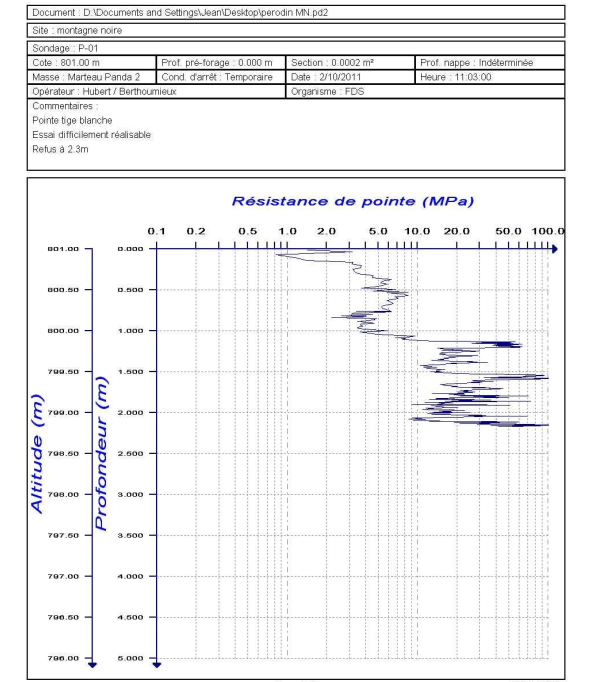
\includegraphics[width=1\textwidth]{./images/penetrographe.png}
    \caption{Exemple de résultat d'un essai pénétrométrique}
    \label{fig:test_penetrometrique}
\end{figure}
